\hypertarget{ux4e0aux4e0bux6587ux4e0eux8bb0ux5fc6}{%
\chapter{上下文与记忆}\label{ux4e0aux4e0bux6587ux4e0eux8bb0ux5fc6}}

\hypertarget{ux6a21ux578bux7684ux8bb0ux5fc6}{%
\section{模型的记忆}\label{ux6a21ux578bux7684ux8bb0ux5fc6}}

\hypertarget{ux4e00ux77edux671fux8bb0ux5fc6ux4e0aux4e0bux6587}{%
\subsection{一、短期记忆（上下文）}\label{ux4e00ux77edux671fux8bb0ux5fc6ux4e0aux4e0bux6587}}

短期记忆是大模型执行任务时对当前任务上下文的记忆，对应``上下文学习''，其底层实现是注意力中存储的KV Cache，任务结束后即清空。

由于硬件显存有限，大模型的上下文窗口长度有限，如果超出长度就必须采取一些机制。对于短期记忆自身而言，可以采取的措施例如：

\begin{enumerate}
\def\labelenumi{\arabic{enumi}.}
\item
  滑动窗口：保留最近的K轮对话。
\item
  摘要：对于更早的内容，生成摘要，并``遗忘''原内容，一般和滑动窗口配合使用。摘要会暂时储存在内存中，并加入后续对话的上下文窗口。
\end{enumerate}

后续还会有和长期记忆配合的一些其他方法。

\hypertarget{ux4e8cux957fux671fux8bb0ux5fc6}{%
\subsection{二、长期记忆}\label{ux4e8cux957fux671fux8bb0ux5fc6}}

我们可以通过向量数据库的形式，将记忆内容嵌入为语义向量，保存在大容量介质（如硬盘）中。例如，OpenClaw将记忆存储在工作区的特定markdown文件中。在运用时，根据请求用向量相似度在数据库中检索，获取最相关的内容，也可以通过提示词让模型以其他方式灵活调取。记忆内容可以包括历史问答及其摘要、垂直领域知识、执行动作的历史及经验教训、用户偏好等。

在上下文超过短期记忆上限时，我们可以将最早的历史信息（或只存其摘要）移动到长期记忆中，在后续如果被检索到（即需要这些信息）则再加入短期记忆。

由于长期记忆读写速度慢，我们一般不会每次对话都访问，而是在初始化（开始工作前）、检索（遇到一定的问题或场景，LLM判断需要调用记忆）或归档（项目做完打包结项）等时候按需要调用。

长期记忆可以分层，如OpenClaw包括一个大数据库和一个精选过的最重要的记忆（如用户偏好、重要决定等），每次涉及与用户对话时都会调取精选记忆。以Claude-mem为例，其采取了``渐进式披露''的方法，在通过检索方法（稠密检索、稀疏检索）得到若干条记忆条目后，不立即全部注入上下文，而是分层处理。具体而言，就是在建立记忆时，就分为如下三层，从而在调用时分层读取：

Layer 1：Search（索引层）：一个``轻量索引''，每一行包括该条记忆的ID、时间、类别、标题、token成本，例如：\textbar{} \#2102\textbar{} Oct 20 \textbar{} problem-solution \textbar{} Fixed timeout in CI \textbar{} 100 tokens \textbar。如gotcha表示这是个坑，problem-solution表示这是曾经的问题与解法等。对于检索到的条目，将它们的索引层注入主模型，模型看标题和类型就能判断：这一条是否有必要调用更贵的Layer 2 / Layer 3。（这里和前面的检索的不同点在于，检索是运用固定的检索算法，因而比较粗略，无法处理精细语义；这里虽然只有少量浓缩信息，但模型可以根据需要灵活判断）

Layer 2：Timeline（时间线层）：事件记忆，类似于日志。当模型在Layer 1中选定ID后，对于每个ID，拉出它的前后几条时间线，看看这步操作的前后都发生了什么。

Layer 3：Get Observations（详情层）：对Layer 1中选定的ID，如果经过读取Layer 2后，模型仍认为需要更多信息，则会拉取该ID对应的完整结构化内容。例如：

\begin{verbatim}
#2543 Hook timeout: 60s too short for npm install

Date: Oct 26, 2025 2:14 PM
Type: gotcha
Project: claude-mem

Narrative:
Discovered that the default 60-second hook timeout is insufficient for npm
install operations, especially with large dependency trees or slow network
conditions. This causes SessionStart hook to fail silently, preventing context
injection.

Facts:
- Default timeout: 60 seconds
- npm install with cold cache: ~90 seconds
- Configured timeout: 120 seconds in plugin/hooks/hooks.json:25

Files Modified:
- plugin/hooks/hooks.json

Concepts: hooks, timeout, npm, configuration
\end{verbatim}

总而言之，这里的结构化信息包括：

Narrative（叙事）：

用自然语言描述``发生了什么、问题是什么、影响是什么''，方便 Agent 理解上下文。

Facts（事实清单）：

关键数值、配置项、结论，方便做逻辑推理。

Files Modified / Files Read：

直接告诉 Agent：这个观察跟哪些文件有关，不用自己去猜。

Concepts（概念标签）：

用于语义检索，例如``hooks / timeout / npm''等，方便后续基于概念检索。

官方示例中，典型的模式是：Layer 1：limit=10条索引；Layer 2：选2--3个ID拉时间线；Layer 3：对于其中有必要的，再完整观察。下面举一个例子：

Layer 1：调用 \texttt{search(\{\ query:\ "hook\ timeout",\ limit:\ 10\ \})}

得到 3 条相关记忆的索引：

\#2543：Hook timeout: 60s too short

\#2891：Hook timeout configuration

\#2102：Fixed timeout in CI

Layer 2：Claude判断\#2543最相关，调用 \texttt{timeline(\{\ anchor:\ 2543,\ depth\_before:\ 3,\ depth\_after:\ 3\ \})}，看到：

之前：尝试过哪些超时配置

当前：把 60s 改成 120s

之后：CI 中也统一了这个配置

Layer 3：如果觉得需要更多细节，再调用 \texttt{get\_observations(\{\ ids:\ {[}2543,\ 2102{]}\ \})}

得到完整的叙事、事实、修改文件列表等，用于当前决策。

\hypertarget{ux4e09ux5185ux5b58}{%
\subsection{三、内存}\label{ux4e09ux5185ux5b58}}

AI Agent（智能体）的运行过程中，系统内存（System RAM / CPU Memory）扮演的是``调度员''和``中转站''的角色，是连接硬盘（数据库）和显卡（LLM）的桥梁。我们写的Agent程序就是在内存中运行的。

对于一些信息，容量超出了短期记忆，但调用频次又较高，难以接受长期记忆的检索效率。因此，我们可以在程序里建立数据结构，在内存里存储。如下面的两个例子。

\begin{enumerate}
\def\labelenumi{\arabic{enumi}.}
\tightlist
\item
  按重要性保留历史信息
\end{enumerate}

设立评分机制（如TF-IDF、注意力权重、打分模型），判断历史信息的重要程度，保留最重要的K条（如K=5或10）内容，适合关键信息分散在较长时间段的任务。

在数据结构的实现上，我们可以在程序中编写一个动态变化的堆，每增加一条对话，就评判其重要性权重，根据分数加入到堆。堆只保留分数最高的K条。当第K+1条数据进来，如果分数不够高，直接丢弃；如果比堆里最低的高，就从堆里去除原来最低的，把它放进去。在下一次问答前，再将堆中的内容加入短期记忆即上下文中。关于为什么这个过程必须在堆而不是上下文里实现，可以参考下面的例子：

你的上下文窗口只能装 3 条记忆。

不使用堆（直接进上下文）：

\begin{enumerate}
\def\labelenumi{\arabic{enumi}.}
\tightlist
\item
  用户说：``我叫小明。'' -\textgreater{} 存入上下文（剩 2 空位）。
\item
  用户说：``今天天气不错。'' -\textgreater{} 存入上下文（剩 1 空位）。
\item
  用户说：``吃个苹果。'' -\textgreater{} 存入上下文（满员）。
\end{enumerate}

突发情况：用户突然说：``我对青霉素过敏！''

此时上下文已经塞满了前 3 条废话。如果要加这条最重要的，你需要复杂的逻辑去``擦除''上下文里的某一条。在 Prompt 字符串里做``查找替换''是非常麻烦且低效的。

在堆里操作：

\begin{itemize}
\tightlist
\item
  操作对象：Python 里的 List/Object。
\item
  代价：纳秒级 CPU 时间，0 块钱。
\item
  灵活性：你可以随意增加、删除、修改权重、重新排序。
\end{itemize}

在上下文里操作：

\begin{itemize}
\tightlist
\item
  操作对象：发给 API 的 Prompt 字符串。
\item
  代价：Token 是按量计费的。一旦你把 Prompt 发出去，就覆水难收。
\end{itemize}

堆（Heap）是草稿纸，上下文（Context）是最终试卷。

\begin{itemize}
\tightlist
\item
  你可以在草稿纸上反复计算、涂改、比较，决定哪道题是重点（在堆里根据分数排序、替换）。
\item
  但是当你把答案写到试卷上（放入 Context Window）并交卷（发送给 LLM）之后，就不能改了。
\end{itemize}

\begin{enumerate}
\def\labelenumi{\arabic{enumi}.}
\setcounter{enumi}{1}
\tightlist
\item
  生成摘要
\end{enumerate}

前面提到过，当对话超出上下文限制时，让LLM为之前的对话生成一段摘要，注入之后的上下文窗口。写成程序语句如\texttt{summary=agent.ask(massage)}，\texttt{massage}里包含了要求生成摘要的prompt，这里的\texttt{summary}就暂时存在内存中，等待被注入新的上下文。

summary并非简单把长文本变成短文本，这会丢失大量细节。它应当保留模型对原始对话的``隐性理解''，就像把一本厚书压缩成一个``记忆卡片''，模型读了卡片就能回忆起整本书的内容。例如OpenAI Codex的策略是，对于代码项目中的对话，当上下文窗口满时，用一个小项目列表替换前文，概括前面都执行了什么。

\hypertarget{ux53c2ux8003ux6587ux732e-133}{%
\subsection{参考文献}\label{ux53c2ux8003ux6587ux732e-133}}

\begin{itemize}
\tightlist
\item
  《动手学大模型智能体》。
\item
  OpenClaw. (2026). \href{https://github.com/openclaw/openclaw}{OpenClaw GitHub repository}.
\item
  thedotmack. (2026). \href{https://github.com/thedotmack/claude-mem}{claude-mem GitHub repository}.
\end{itemize}

\clearpage

\hypertarget{ux4e0aux4e0bux6587ux7ba1ux7406}{%
\section{上下文管理}\label{ux4e0aux4e0bux6587ux7ba1ux7406}}

\hypertarget{ux4e00ux63d0ux9ad8ux7f13ux5b58ux547dux4e2dux7387}{%
\subsection{一、提高缓存命中率}\label{ux4e00ux63d0ux9ad8ux7f13ux5b58ux547dux4e2dux7387}}

对于Agent Loop来说，每跑一圈都要把之前的对话历史（包括那些冗长的报错信息、文件内容）重新发给模型，将导致计算复杂度平方级增长。可以采用缓存策略让KV Cache尽可能命中。

从缓存角度，上下文从前到后往往分为：全局缓存（System指令、工具定义）；任务/项目级缓存（如CLAUDE.md，AGENT.md）；会话级缓存（历史对话）；当前会话消息（用户输入、环境反馈结果等）。尽量把静态内容放在前面，动态内容放在后面。对于前面不变的部分，服务器就不需要重新计算，直接调取缓存中的历史记录。

这样可以让长对话的成本从平方级增长降到线性级。但任何改变System指令/工具定义/历史对话等的操作都会导致缓存失效，如中途换模型、切换工作目录、修改权限配置、改变MCP工具列表等。为尽可能确保缓存命中，有以下方法：

\begin{enumerate}
\def\labelenumi{\arabic{enumi}.}
\item
  保持提示前缀稳定。由于LLM的自回归特性，即使是单个标记的差异也会使该标记之后的缓存失效。例如，一些配置修改、工具变更尽量通过在input中附加一条信息，如system propmt的修改可用类似于的形式实现，而非完全抛弃缓存。一个常见的错误是在系统提示的开头包含时间戳，尤其是精确到秒的时间戳，这会大大降低缓存命中率。
\item
  使会话上下文只追加。避免修改之前的操作或观察。要当心的是许多编程语言和库在序列化JSON对象时不保证键顺序的稳定性，这可能会悄无声息地破坏缓存。上下文精简尽量在缓存本来就要未命中的时候进行。
\item
  在需要时明确标记缓存断点。某些模型提供商或推理框架不支持自动增量前缀缓存，而是需要在上下文中手动插入缓存断点。在分配这些断点时，要考虑潜在的缓存过期问题，并至少确保断点包含系统提示的结尾。
\end{enumerate}

\begin{figure}[htbp]
\centering
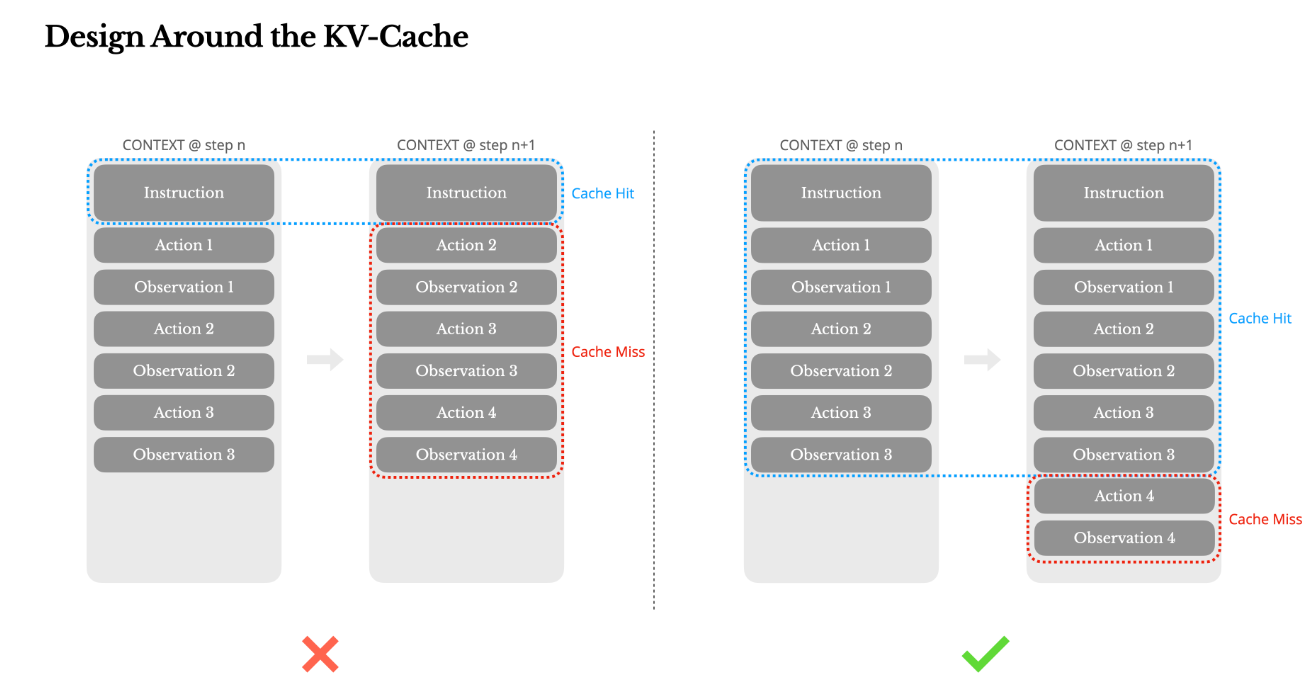
\includegraphics{images/image-0035.png}
\caption{KV Cache 缓存命中与未命中对比}
\end{figure}

\hypertarget{ux4e8cux5de5ux5177ux7ba1ux7406}{%
\subsection{二、工具管理}\label{ux4e8cux5de5ux5177ux7ba1ux7406}}

随着Agent能力的增强，其行动空间自然变得更加复杂，即工具数量爆炸式增长。如果允许用户自定义工具，总会有人将数百个神秘工具插入到行动空间中。结果，模型更可能选择错误的行动或采取低效的路径，Agent变得更加愚蠢。

一个自然的反应是设计一个动态行动空间，使用类似于RAG的方法按需加载工具，上下文中只包含这些被加载的工具。但实验表明，除非绝对必要，避免在迭代过程中动态添加或移除工具。这一方面是因为工具定义在上下文的前部，任何更改都会使后续所有动作和观察的KV缓存失效，另一方面是因为当先前的动作和观察仍然引用当前上下文中不再定义的工具时，模型会感到困惑，如果没有约束解码，这通常会导致模式违规或幻觉动作。

为了解决这个问题并仍然改进动作选择，有以下方法：

\begin{enumerate}
\def\labelenumi{\arabic{enumi}.}
\tightlist
\item
  只在上下文保留``元工具''，调用这些元工具会将模型导引到文件系统中具体工具存储的位置。这种设计本质上也是渐进式披露，好处在于让工具灵活且可扩展。
\end{enumerate}

以Claude Code的skills为例，技能存储在文件系统中，而非绑定工具，Claude只需调用几个简单的函数（如Bash、文件系统）即可逐步发现和使用技能，然后让模型自主提取需要的技能使用。这个过程只涉及会话上下文的累积，而不涉及上下文最前面工具定义的变化。

Manus也是如此，它只保留了不到20个``原子函数（Atomic Functions）''，如执行Bash命令、读写文件、执行Python代码。复杂的业务逻辑被包装成了沙盒里的CLI（命令行程序），模型不需要知道这几百个MCP工具的JSON Schema。模型只需要知道``我会用Bash''。当它需要使用MCP工具时，它直接在Bash工具里输入类似mcp-cli run some\_tool的命令即可。这里也不需要通过语义相似度的向量索引进行检索。

\begin{enumerate}
\def\labelenumi{\arabic{enumi}.}
\setcounter{enumi}{1}
\item
  只保留工具列表，让模型在需要的时候在文件系统中检索工具定义。GPT-5.4采取的就是这种策略。
\item
  在需要移除工具时，不直接将工具移出上下文，而是在解码过程中掩蔽token的logits，以基于当前上下文阻止（或强制）选择某些动作，或者通过prompt要求模型禁止使用特定工具（但这本质上变成了注意力机制的博弈，模型仍然有概率``违规操作''生成被禁用的工具）。
\end{enumerate}

\begin{figure}[htbp]
\centering
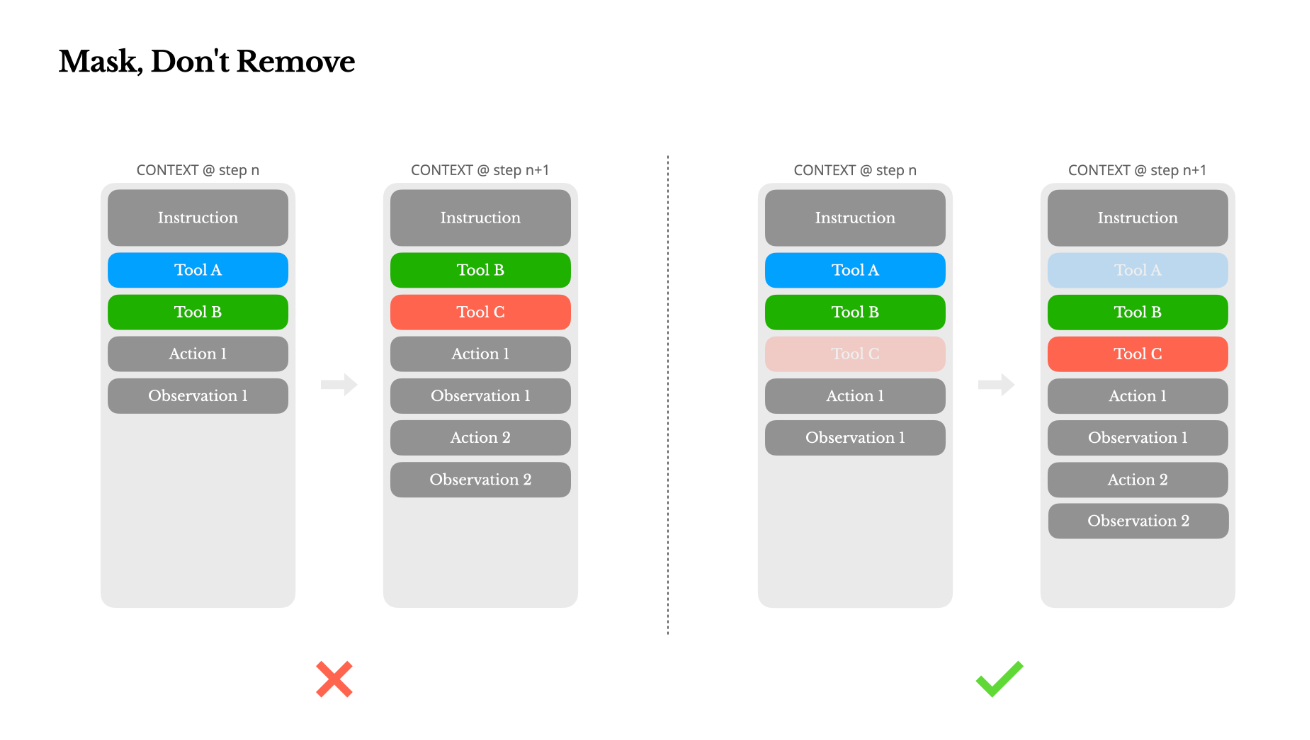
\includegraphics{images/image-0036.png}
\caption{掩蔽工具而不是从上下文移除工具}
\end{figure}

函数调用通常有三种模式：

自动：模型可以选择调用或不调用函数。通过仅预填充回复前缀实现：\textless\textbar im\_start\textbar\textgreater assistant

必需：模型必须调用函数，但选择不受约束。通过预填充到工具调用令牌实现：\textless\textbar im\_start\textbar\textgreater assistant

指定：模型必须从特定子集中调用函数。通过预填充到函数名称的开头实现：\textless\textbar im\_start\textbar\textgreater assistant\{``name'': ``browser\_''\}

\hypertarget{ux4e09ux4e0aux4e0bux6587ux7a97ux53e3-ux6587ux4ef6ux7cfbux7edfux5206ux5c42ux7ed3ux6784}{%
\subsection{三、``上下文窗口-文件系统''分层结构}\label{ux4e09ux4e0aux4e0bux6587ux7a97ux53e3-ux6587ux4ef6ux7cfbux7edfux5206ux5c42ux7ed3ux6784}}

上下文窗口有限，而信息的压缩是不可逆的。为此，我们可以只将重要信息留存在上下文窗口，其余则存储在文件系统中。模型学会按需写入和读取文件，不仅将文件系统用作存储，还用作结构化的外部记忆。

\begin{figure}[htbp]
\centering
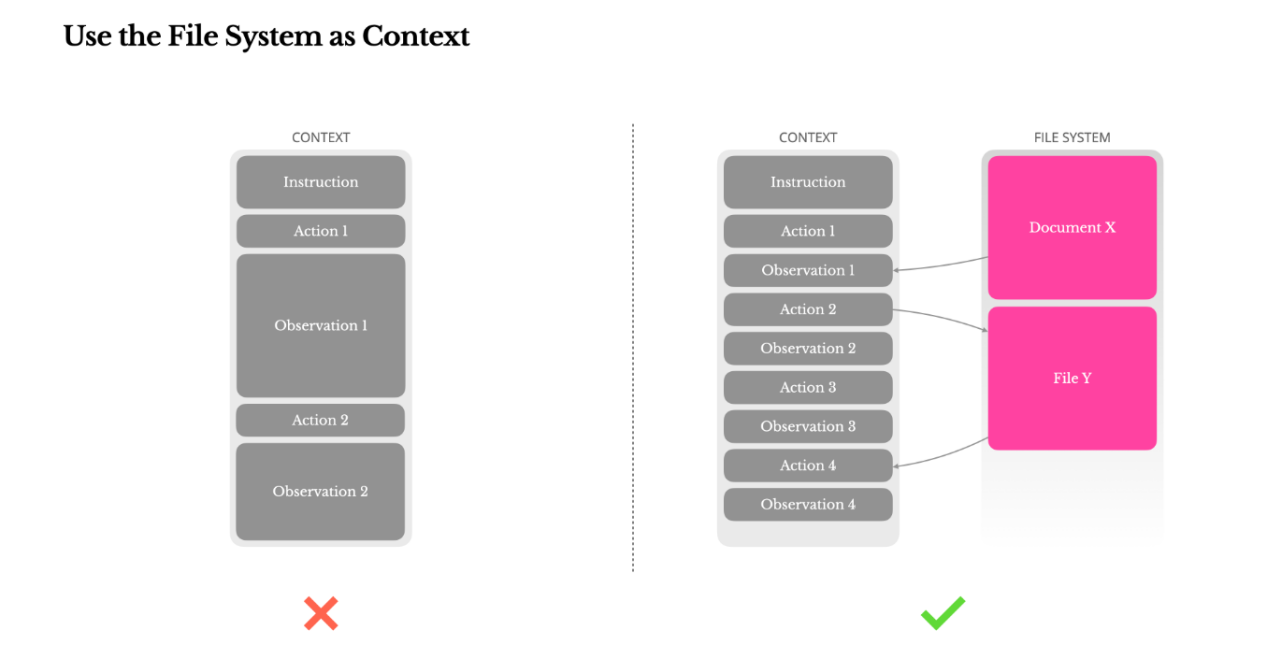
\includegraphics{images/image-0037.png}
\caption{将文件系统作为上下文}
\end{figure}

当上下文将满时，模型触发压缩（即在上下文最后加一条消息表示需要压缩）。对于工具调用结果，除了本轮会话以外，前面各轮会话的工具调用结果都会被压缩为指向文件系统中对应内容的索引。

\begin{figure}[htbp]
\centering
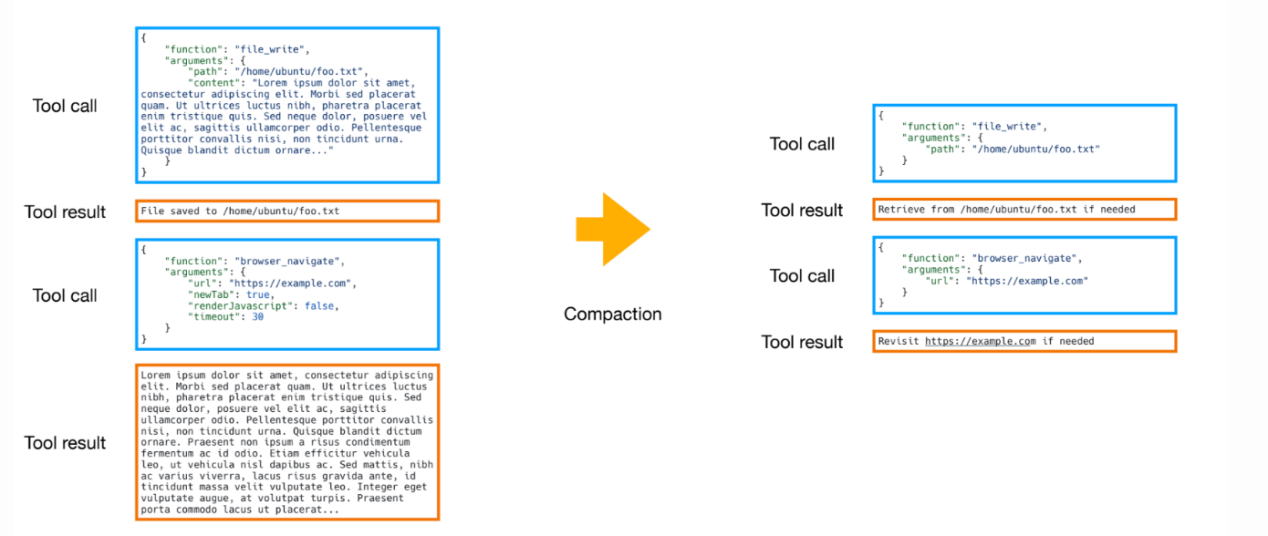
\includegraphics{images/image-0038.png}
\caption{将工具调用结果压缩为文件系统引用}
\end{figure}

\hypertarget{ux56dbux590dux8ff0ux76eeux6807}{%
\subsection{四、复述目标}\label{ux56dbux590dux8ff0ux76eeux6807}}

在处理复杂任务时，很多Agent会倾向于创建类似于todo.md的计划文件，并在任务进行过程中逐步更新它，勾选已完成的项目。这不仅是为了方便用户审阅，更重要的是，这是在操控注意力，通过将其目标复述到上下文的末尾的方式，避免模型在复杂任务后期偏离目标。

\begin{figure}[htbp]
\centering
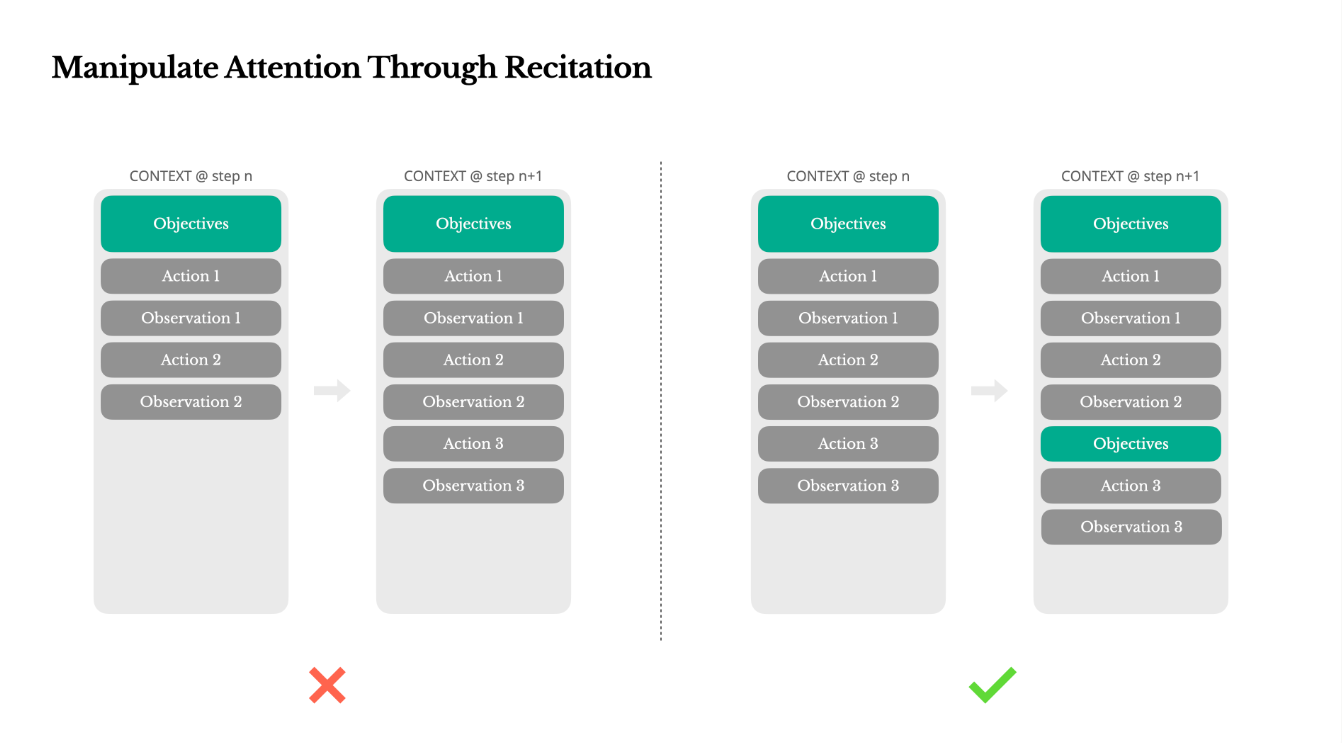
\includegraphics{images/image-0039.png}
\caption{通过复述目标操控注意力}
\end{figure}

\hypertarget{ux4e94ux4e0dux8981ux88abux5c11ux6837ux672cux793aux4f8bux6240ux56f0}{%
\subsection{五、不要被少样本示例所困}\label{ux4e94ux4e0dux8981ux88abux5c11ux6837ux672cux793aux4f8bux6240ux56f0}}

语言模型是优秀的模仿者；它们模仿上下文中的行为模式。如果上下文充满了类似的过去行动-观察对，模型将倾向于遵循该模式，即使这不再是最优的。这在涉及重复决策或行动的任务中可能很危险。例如，当审查20份简历时，代理通常会陷入一种节奏，即仅仅因为这是它在上下文中看到的，就重复与之类似的行动。这导致偏离、过度泛化，或有时产生幻觉。

解决方法是增加多样性，在行动和观察中引入少量的结构化变化，如不同的序列化模板、替代性措辞、顺序或格式上的微小噪音。这种受控的随机性有助于打破模式并调整模型的注意力。

\begin{figure}[htbp]
\centering
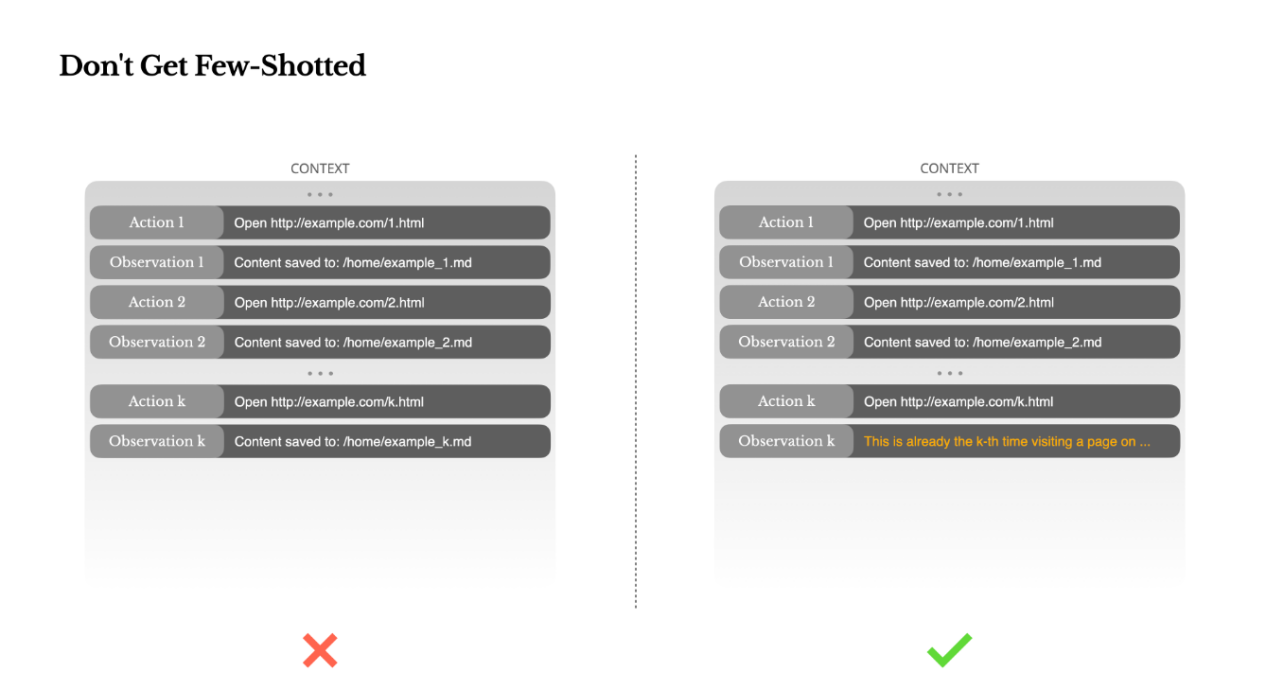
\includegraphics{images/image-0040.png}
\caption{避免少样本示例锁定行为模式}
\end{figure}

\hypertarget{ux516dux591aux667aux80fdux4f53ux7684ux4e0aux4e0bux6587ux9694ux79bb}{%
\subsection{六、多智能体的上下文隔离}\label{ux516dux591aux667aux80fdux4f53ux7684ux4e0aux4e0bux6587ux9694ux79bb}}

在多智能体系统中，主Agent和子Agent（如分别作为规划器和执行器）的上下文会存在一定隔离，如二者的system prompt和tools定义不同的。其余上下文可以不共享，但长上下文的复杂任务中仍建议共享。

不共享的范式：

\begin{figure}[htbp]
\centering
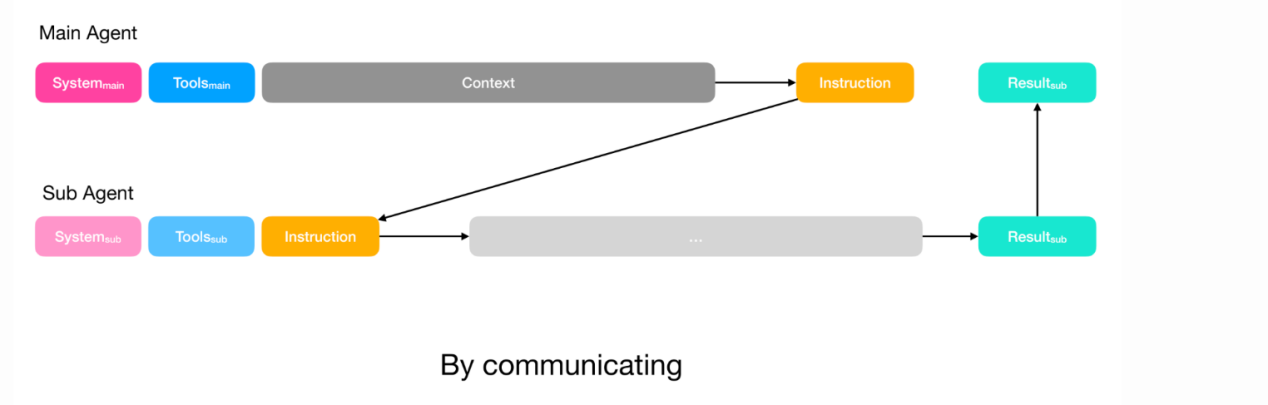
\includegraphics{images/image-0041.png}
\caption{主 Agent 与子 Agent 通过通信隔离上下文}
\end{figure}

部分共享的范式：（如主Agent作为规划者，与子Agent共享完整的上下文，子Agent仍拥有自己的动作空间（工具）和指令，但会获得规划者同样可访问的完整上下文。）

\begin{figure}[htbp]
\centering
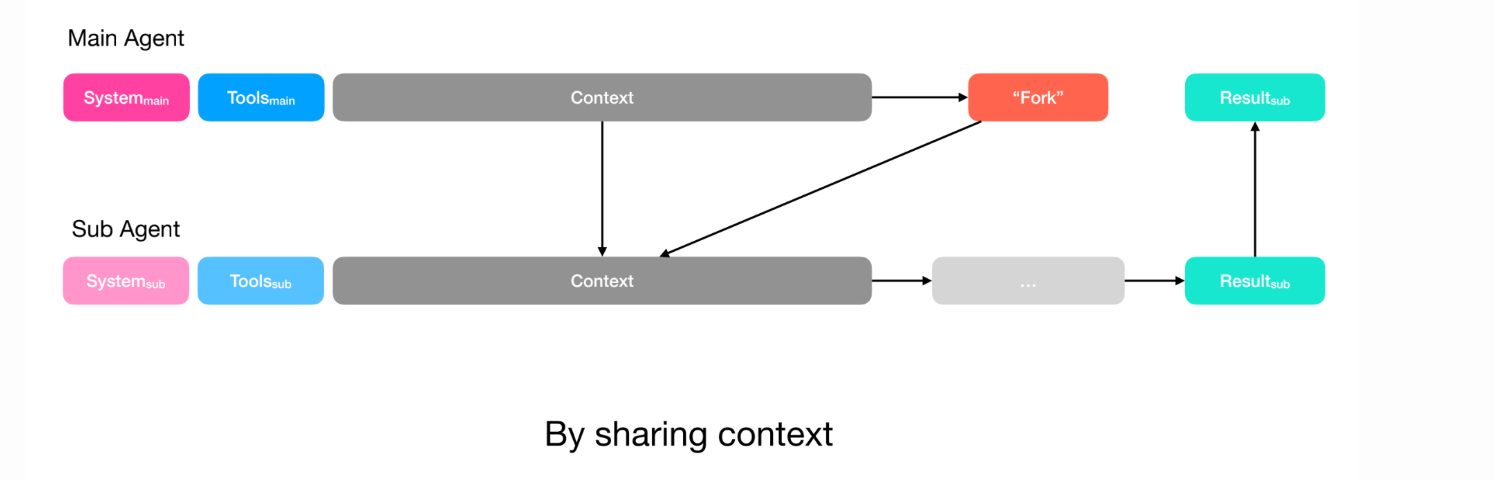
\includegraphics{images/image-0042.png}
\caption{主 Agent 与子 Agent 共享上下文}
\end{figure}

在这两种情况下，规划者都定义了子代理的输出模式。子代理有工具在返回结果前填充该模式，Manus 则使用约束解码确保输出符合定义模式。\texttt{submit\ results}

\hypertarget{ux53c2ux8003ux6587ux732e-134}{%
\subsection{参考文献}\label{ux53c2ux8003ux6587ux732e-134}}

\begin{itemize}
\tightlist
\item
  Martin, L. (2025). \href{https://rlancemartin.github.io/2025/10/15/manus/}{Context Engineering for Agents}.
\item
  Manus. (2025). \href{https://manus.im/zh-cn/blog/Context-Engineering-for-AI-Agents-Lessons-from-Building-Manus}{Context Engineering for AI Agents: Lessons from Building Manus}.
\end{itemize}

\clearpage

\hypertarget{ux57faux4e8eux6ce8ux610fux529bux5339ux914dux7684kvux538bux7f29ux8bbaux6587}{%
\section{基于注意力匹配的KV压缩（论文）}\label{ux57faux4e8eux6ce8ux610fux529bux5339ux914dux7684kvux538bux7f29ux8bbaux6587}}

\begin{quote}
本文是论文阅读笔记，内容代表对应论文方法或作者理解，不应直接视为领域共识或工程最佳实践。
\end{quote}

\hypertarget{ux4e00ux63d0ux51faux80ccux666f-3}{%
\subsection{一、提出背景}\label{ux4e00ux63d0ux51faux80ccux666f-3}}

在长上下文场景中，将长上下文总结为短文本虽然常用，但会丢失大量信息；在潜在空间训练紧凑KV缓存的方法（如Cartridges方法）能保持高性能，但需要昂贵的端到端梯度优化，耗时极长，通常需要数小时GPU算力才能压缩一个上下文。于是，我们希望不依赖于端到端的输出概率优化，而是直接优化紧凑的键和值，使其在每一个KV头上，对于每一个query，尽可能复现原始的``注意力输出''和``注意力质量（Attention Mass）''。

\hypertarget{ux4e8cux6838ux5fc3ux601dux60f3-3}{%
\subsection{二、核心思想}\label{ux4e8cux6838ux5fc3ux601dux60f3-3}}

该方法的核心思想是：不依赖于端到端的输出概率优化，而是直接优化紧凑的键和值，使其在每一个 KV 头上，尽可能复现原始的``注意力输出''和``注意力质量（Attention Mass）''。

假设原始上下文有 \(T\) 个 token，其键和值为 \(K,V \in \mathbb{R}^{T \times d}\)，我们要将其压缩为长度为 \(t\)（其中 \(t<T\)）的紧凑缓存 \(C_k,C_v \in \mathbb{R}^{t \times d}\)。为了补偿压缩后注意力总量的流失，作者引入了一个每个 token 标量偏差（Scalar Bias）\(\beta \in \mathbb{R}^{t}\)。

给定一组参考查询（Reference Queries）\(q \in \mathbb{R}^{1 \times d}\)，我们需要同时满足以下两个数学目标：

\begin{enumerate}
\def\labelenumi{\arabic{enumi}.}
\tightlist
\item
  匹配局部注意力输出（Local Attention Output）：
\end{enumerate}

\[
\frac{\exp(qK^\top)V}{\sum_{j=1}^{T}\exp(qK_j^\top)}
\approx
\frac{\exp(qC_k^\top+\beta)C_v}{\sum_{j=1}^{t}\exp(q(C_k)_j^\top+\beta_j)}
\]

这是为了对于 query，经过上下文聚合后输出的结果不变。

\begin{enumerate}
\def\labelenumi{\arabic{enumi}.}
\setcounter{enumi}{1}
\tightlist
\item
  匹配注意力质量（Attention Mass）：
\end{enumerate}

\[
\sum_{j=1}^{T}\exp(qK_j^\top)
\approx
\sum_{j=1}^{t}\exp(q(C_k)_j^\top+\beta_j)
\]

这是为了确保被压缩后的旧上下文，在未来遇到新输入的 token 时，依然能保持与原始完整上下文同等的``话语权''或``权重占比''。

传统的上下文压缩方法（如 Token 丢弃、KVzip 等）通常只是从 \(T\) 个 token 中挑出 \(t\) 个重要的 token 留下来（\(t<T\)）。

因为指数函数 \(\exp(x)\) 永远大于 0，所以保留 \(t\) 个 token 的 Mass 必然会系统性地小于原始 \(T\) 个 token 的 Mass：

\[
\sum_{j=1}^{t}\exp(q(C_k)_j^\top)
<
\sum_{j=1}^{T}\exp(qK_j^\top)
\]

当你用这种粗暴的压缩方法后，一旦系统追加了新的 token（\(K_{fixed}\)），由于压缩块的 Mass 变小了，它在上述加权混合公式中的占比就会骤降。模型会不成比例地把注意力过度集中在``新 token''上，从而在数学层面上被动地``遗忘''或``忽视''了被压缩的历史上下文。

一个通俗的类比：股东大会代表制。

\begin{itemize}
\tightlist
\item
  原始情况：公司有 1000 个小股东（原始 \(T\) 个 token），每人 1 票，总投票权（Attention Mass）为 1000。
\item
  传统压缩（丢弃法）：选出 50 个核心股东代表去开会，其他人不去。如果按人头算，旧股东阵营的总投票权骤降到 50。当有新投资人（new token）带着 100 票入场时，旧股东阵营的话语权会被彻底稀释。
\item
  匹配注意力质量（论文做法）：同样选出 50 个代表（挑选 \(C_k\)），但是赋予他们``代理投票权''（标量偏差 \(\beta\)），比如代表 A 身上背了 20 个人的票，代表 B 身上背了 30 个人的票。这样虽然人少了，但旧阵营的总票数依然是 1000（Mass 匹配）。当新投资人进来时，旧阵营的决策影响力（局部注意力输出）和话语权占比（混合权重）依然完美保持不变。
\end{itemize}

\hypertarget{ux4e09ux7b97ux6cd5ux6d41ux7a0b}{%
\subsection{三、算法流程}\label{ux4e09ux7b97ux6cd5ux6d41ux7a0b}}

共分3个步骤：采样参考查询（\(Q_{\mathrm{ref}}\)）；选择保留的键（\(C_k\)）并拟合偏差（\(\beta\)）；得到值（\(C_v\)）。

\hypertarget{ux4e00step1ux91c7ux6837ux53c2ux8003ux67e5ux8be2q_mathrmref}{%
\subsubsection{\texorpdfstring{（一）Step1：采样参考查询（\(Q_{\mathrm{ref}}\)）}{（一）Step1：采样参考查询（Q\_\{\textbackslash mathrm\{ref\}\}）}}\label{ux4e00step1ux91c7ux6837ux53c2ux8003ux67e5ux8be2q_mathrmref}}

对于不同的查询 \(Q\)，模型在用这些 \(Q\) 查询原文时，为了保证语法的连贯性、指代的准确性以及语义的连贯，会同时把注意力分散到历史中的多个关键 token 上。那些在不同 \(Q\) 下多次获得较高注意力分数的关键词，就是高价值的、需要保留的信息。我们无法预知未来的用户提问，也就不知道未来的 \(Q\) 分布，故我们希望诱导模型生成高质量的 \(Q\)。有以下两种方法：

\begin{enumerate}
\def\labelenumi{\arabic{enumi}.}
\tightlist
\item
  Repeat-prefill（重复预填充）
\end{enumerate}

它的具体做法是构造这样一个特殊的输入序列送给模型：

\begin{verbatim}
"[原始长文本 C] 接下来，请一字不差地重复前面的文本：[再次输入原始长文本 C]"
\end{verbatim}

内部重构时的``疯狂回看''：当模型在预填充（Prefill）阶段处理到第二个 \texttt{\{C\}} 时，为了准确预测下一个词，当前 token 的 \(Q\) 向量必须极度精准地去匹配第一个 \texttt{\{C\}} 中对应位置的 \(K\) 向量。这就好比你在抄写一段长文，你的眼睛（Query）会不断地、强烈地去回看原稿（Key）。

提取参考查询：这个``回看''过程中产生的 \(Q\) 向量，完美代表了``当模型真正需要从长上下文中精确提取细节时，它会发出怎样的查询请求''。

提取出来：在代码层面，我们只是在模型前向传播（Forward Pass）经过这些特定 token 时，把某些层注意力头里计算出的 \(Q\) 矩阵直接拷贝并保存下来。这些真实且高质量的 \(Q\) 就构成了我们的``参考查询集（\(Q_{ref}\)）''，作为后续压缩算法的``靶子''。

当大模型在输出``哪怕是一个完全`照抄'的词''时，它为了保证语法的连贯性、指代的准确性以及语义的连贯，其内部的 Query 向量会同时把注意力分散到历史中的多个关键节点上。

\begin{itemize}
\tightlist
\item
  举个例子：原文如果是``苹果公司在今天的发布会上，揭出了一部全新的手机。''
\item
  当模型在``重复''生成``手机''这个词时，它的 \(Q\) 向量不仅会去看原文末尾的``手机''，还会分配大量的注意力去看``苹果公司''、``库克''和``发布会''。因为模型需要这些上下文来确定当前语境。
\item
  结果就是：像``苹果公司''、``库克''这样的核心实体词（Key），会在模型重复整段话的过程中，被无数个后续生成的词的 \(Q\) 反复``回看''和依赖。
\end{itemize}

\begin{enumerate}
\def\labelenumi{\arabic{enumi}.}
\setcounter{enumi}{1}
\tightlist
\item
  Self-study（自学/自我提问）
\end{enumerate}

这是一种基于合成数据的方法。我们将原始上下文 \texttt{\{C\}} 喂给模型，并给它下一些指令（例如``总结关键事实''或``根据上下文提出 3 个问题''），让模型自己生成对话或问答。在模型``生成响应（Decoding）''的过程中，提取其注意力头产生的查询向量。这模拟了真实下游推理任务中查询向量的分布。

\hypertarget{ux4e8cstep2ux9009ux62e9ux4fddux7559ux7684ux952ec_kux5e76ux5229ux75282ux5f0fux62dfux5408ux504fux5deebeta}{%
\subsubsection{\texorpdfstring{（二）Step2：选择保留的键（\(C_k\)）并利用（2）式拟合偏差（\(\beta\)）}{（二）Step2：选择保留的键（C\_k）并利用（2）式拟合偏差（\textbackslash beta）}}\label{ux4e8cstep2ux9009ux62e9ux4fddux7559ux7684ux952ec_kux5e76ux5229ux75282ux5f0fux62dfux5408ux504fux5deebeta}}

只有一定数量的 token 会被保留，它们的键构成 \(C_k\)。这一步选择保留哪些 token（即保留哪些键）。有以下两种方法：

\begin{enumerate}
\def\labelenumi{\arabic{enumi}.}
\tightlist
\item
  保留最高注意力键并拟合偏差
\end{enumerate}

计算局部注意力分数：针对每一个参考查询 \(q_i\)，计算其在所有原始键 \(K\) 上的 Softmax 注意力分布：

\[
a_i = \mathrm{softmax}(q_i K^\top) \in \mathbb{R}^{1 \times n}
\]

跨查询聚合打分：对于第 \(j\) 个键，它在 \(n\) 个不同查询下会得到 \(n\) 个分数 \((a_{1,j}, a_{2,j}, \ldots, a_{n,j})\)。通过计算这些分数的均方根（Root Mean Square, RMS），得到该键的全局重要性得分 \(s_j\)。

排序与截断：根据 \(s_j\) 对所有原始键进行降序排列，直接提取 Top-\(t\) 个键构成 \(C_k\)。
在选择好一定数量键后，为保证注意力质量不变，根据（2）式，需要加上偏差。

我们的根本目标是让压缩后的缓存，在任意查询 \(q_i\) 下，其``注意力质量''等于原始缓存的质量 \(m_i\)：

\[
m_i = \sum_{j=1}^{T} \exp(q_i K_j^\top)
\]

为了用少量的 \(t\) 个键（\(C_k\)）凑出原本庞大的质量 \(m_i\)，作者为每个选中的键引入了一个待学习的标量偏差（Scalar Bias）\(\beta_j\)。近似等式变为：

\[
m_i \approx \sum_{j=1}^{t} \exp(q_i (C_k)_j^\top + \beta_j)
\]

根据指数函数的性质 \(\exp(A + B) = \exp(A)\exp(B)\)，我们可以将上式拆解为：

\[
m_i \approx \sum_{j=1}^{t} \exp(\beta_j) \cdot \exp(q_i (C_k)_j^\top)
\]

此时，我们定义一个新变量 \(w_j = \exp(\beta_j)\)。由于任何实数的指数都必定大于 0，所以这里的 \(w_j\) 隐含了一个严格的物理约束：它必须是非负的（\(w_j > 0\)，或放宽至 \(w_j \ge 0\)）。等式变形为：

\[
m_i \approx \sum_{j=1}^{t} w_j \exp(q_i (C_k)_j^\top)
\]

我们将所有参考查询上的方程联立，写成矩阵形式。令矩阵 \(A_{ij} = \exp(q_i (C_k)_j)\)，权重向量 \(w = [w_1,\ldots,w_t]^\top\)，目标向量为 \(m\)。上面的方程组就可以简洁地表示为：

\[
Aw \approx m
\]

为了找到最能让等式成立的 \(w\)，我们最小化等式两边的几何距离（L2 范数），并带入前面推导出的非负约束。这就构成了经典的 NNLS 目标函数：

\[
\min_{w \ge 0}\|Aw - m\|_2^2
\]

\begin{itemize}
\tightlist
\item
  固定选好的 \(C_k\) 后，目标是求解权重向量 \(w\)（其中 \(w_j = \exp(\beta_j)\)）以匹配目标注意力质量 \(m\)。
\item
  这被转化为一个非负最小二乘（NNLS）优化问题：\(\min_{w \ge 0}\|Aw - m\|_2^2\)。
\item
  求解后取对数得到 \(\beta_j = \log(w_j)\)。直观上，\(w_j\) 代表保留下来的紧凑键``代理''了多少个原始键的注意力质量。
  但这种``选择得分最高的键''的策略的盲区在于忽视了键与键之间的相关性和重叠度。假设组建一支5人的篮球队，如果按``个体最高得分''来选，你可能会选出联盟里得分最高的5个中锋。他们每个人的绝对实力都极强（注意力分数极高），但把他们放在一个队里，由于位置和技能高度重合（信息冗余），球队根本无法运转。
\end{itemize}

在LLM的注意力机制中，如果原文中有两个表达相似概念的词，或者同一句话中的两个强关联 token，它们可能会在参考查询下同时获得极高的注意力分数。如果采用最高分数策略，算法会把这两个高度冗余的键都选进来，浪费了原本就极其稀缺的压缩容量。

\begin{enumerate}
\def\labelenumi{\arabic{enumi}.}
\setcounter{enumi}{1}
\tightlist
\item
  正交匹配追踪（Orthogonal Matching Pursuit, OMP）
\end{enumerate}

假设你想调配出一种极其复杂的特定颜色（目标注意力质量 \(m\)），但你手头有上万种基础颜料（原始的所有键 \(K\)），而由于成本限制，你最终只能挑出其中的 \(t\) 种来混合（预算 \(t\) 个紧凑键）。

OMP 采用的是一种贪心且不断自我修正的策略：

\begin{enumerate}
\def\labelenumi{\arabic{enumi}.}
\item
  贪心寻找：每次找都去盯着当前调出来的颜色和目标颜色之间的``色差''（残差）。在剩下的颜料里，挑出一种与这个``色差''最接近、最能弥补当前差距的颜料。
\item
  正交投影（重拟合）：每次挑入新颜料后，不能只管新加的，而是要把目前挑出来的所有颜料重新按比例混合一次（重新计算权重 \(w\)），以确保当前的混合方案在数学上是``最优解''（即残差与当前所选特征空间正交，误差最小）。
  这样，我们每次都取在语义上互补的键，就能尽可能覆盖全面的信息，不出现重复。
\item
  初始化阶段：计算原始上下文的``目标注意力质量向量'' \(m\)。设定初始残差 \(r = m\)（一开始差距最大），并将``已选键集合'' \(S\) 设为空集。
\item
  计算相关性（Compute Correlation）：遍历所有目前还没有被选中的原始键 \(j \notin S\)。计算当前残差 \(r\) 与该键对应的特征列 \(\Phi_{:,j}\) 之间的内积：
\end{enumerate}

\[
c_j = r^\top \Phi_{:,j}
\]

内积越大，说明这个键越能解释剩下的残差。

\begin{enumerate}
\def\labelenumi{\arabic{enumi}.}
\setcounter{enumi}{2}
\tightlist
\item
  贪心选择（Greedy Selection）：在所有未选的键中，找出相关性得分最高（也就是最对口）的那个键 \(j^\star\)，把它正式纳入已选集合 \(S\) 中：
\end{enumerate}

\[
S \leftarrow S \cup \{j^\star\}
\]

\begin{enumerate}
\def\labelenumi{\arabic{enumi}.}
\setcounter{enumi}{3}
\tightlist
\item
  重拟合权重（Refit Weights via NNLS）：这一步是 OMP 的灵魂。现在 \(S\) 里面有了新成员，我们需要对 \(S\) 中所有的键重新分配``代理权重''（标量偏差）。我们通过求解一个非负最小二乘（NNLS）问题，找到一组非负权重 \(w\)，使得它们组合起来最接近目标 \(m\)：
\end{enumerate}

\[
w \leftarrow \arg\min_{w \ge 0}\|\Phi_{:,S}w - m\|_2^2
\]

\begin{enumerate}
\def\labelenumi{\arabic{enumi}.}
\setcounter{enumi}{4}
\tightlist
\item
  更新残差（Update Residual）：用目标向量减去当前已拟合出的结果，计算出最新的残差：
\end{enumerate}

\[
r \leftarrow m - \Phi_{:,S}w
\]

这也可以视为从m向已有键构成的超平面作投影，找到残差。

\begin{enumerate}
\def\labelenumi{\arabic{enumi}.}
\setcounter{enumi}{5}
\tightlist
\item
  循环迭代：重复步骤 2 到步骤 5，每轮挑一个键，直到集合 \(S\) 中塞满了我们预设的 \(t\) 个键为止。
\end{enumerate}

\hypertarget{ux4e09step3ux5f97ux5230ux503ccv}{%
\subsubsection{（三）Step3：得到值（Cv）}\label{ux4e09step3ux5f97ux5230ux503ccv}}

现在 \(\beta\) 和 \(C_k\) 都确定了。由于加上了偏差 \(\beta\)，为保证注意力输出不变，根据（1）式，被选中的 token 的 \(C_v\) 不会等于其原来的 \(V\) 值。对于第 \(i\) 个测试查询，注意力输出 \(y_i\) 满足：

\[
y_i =
\frac{\exp(q_i K^\top)V}{\sum_{j=1}^{T}\exp(q_i K_j^\top)}
\]

在我们的压缩模型中，既然 \(C_k\) 和 \(\beta\) 已经固定，那么对于查询 \(q_i\)，它在压缩键上产生的归一化注意力权重也就彻底固定了。我们把它记为 \(x_i \in \mathbb{R}^{1 \times t}\)：

\[
x_i =
\frac{\exp(q_i C_k^\top + \beta)}{\sum_{j=1}^{t}\exp(q_i (C_k)_j^\top + \beta_j)}
\]

我们要寻找一个新的紧凑值矩阵 \(C_v \in \mathbb{R}^{t \times d}\)，使得它在权重 \(x_i\) 的加权下，输出的结果尽可能等于原始目标 \(y_i\)：

\[
x_i C_v \approx y_i
\]

那么，整个优化问题就变成了一个极其标准的普通线性回归（Ordinary Least Squares, OLS）：

\[
XC_v \approx Y
\]

我们要最小化它的 L2 误差：

\[
C_v = \arg\min_{C_v}\|XC_v - Y\|_2^2
\]

熟悉线性代数的话，可以直接写出它的解析解（正规方程）：

\[
C_v = (X^\top X)^{-1}X^\top Y
\]

\hypertarget{ux53c2ux8003ux6587ux732e-135}{%
\subsection{参考文献}\label{ux53c2ux8003ux6587ux732e-135}}

\begin{itemize}
\tightlist
\item
  Zweiger, A., Fu, X., Guo, H., \& Kim, Y. (2026). \href{https://arxiv.org/abs/2602.16284}{Fast KV Compaction via Attention Matching}. arXiv:2602.16284.
\end{itemize}

\clearpage
